\documentclass[UTF8]{ctexart}
\usepackage{graphicx}
\usepackage{amssymb}
\usepackage{subfiles}
\usepackage{amsmath}
\usepackage[margin=1in]{geometry}
\title{vtk文件格式}
\begin{document}
\maketitle
\paragraph{\quad}可视化工具包(vtk)提供了许多源和编写器对象对流行的数据文件格式进行读写。
                vtk也提供一些其自己的文件格式。创建另一种文件格式的目的在于为多种数据集
                提供一致的数据表示方案以及简单的软件间数据通信方式。当可能时,我们建议使
                用更广泛使用的文件格式。相反,这里描述的vtk格式可以代替使用。注意其他工具
                可能不支持这些格式。
\paragraph{\quad}vtk中有两种不同的文件格式。最简单的是传统的串行格式,其易于以手动或程序方
                式读写。


\section*{simple legacy formats-简单传统格式}

\paragraph{\quad}传统vtk格式包含五个部分。
\begin{enumerate}
    \item 第一个部分是文件的版本和标识符。这一部分包含单行:'# vtk DataFile version x.x'.
          除版本号x.x外,这一行必须如所示完全一致,而版本数随vtk发行版变化而变化(注:当前版本
          数为3.0,版本1.0和版本2.0与版本3.0文件兼容)
    \item 第二个部分是标题。标题由以结束符'\n'结尾的字符串组成。其最大字符数为256。它可用于描述
          数据和其他任何相关信息。
    \item 下一部分是文件格式。该文件格式描述文件的类型是ASCII或二进制文件。单词ASCII或BINARY
          必须出现在这一行。
    \item 第四部分为数据结构。几何部分描述了数据集的几何与拓扑。这一部分包含以DATASET开头的关键字
          的以及其后描述数据集类型的关键字的单行组成。随后,根据数据集的类型,其他关键字/数据组合
          定义了真实数据。
    \item 最后一部分描述数据集的属性。这一部分以关键字POINT_DATA或者CELL_DATA开始,后跟一个整数
          分别表示点或单元的数量。POINT_DATA或CELL_DATA谁先出现不重要。其他关键字/数据组合定义
          真实数据集的属性值(如标量,向量,张量,发现,纹理坐标或场量)。
\end{enumerate}
\paragraph{\quad}文件格式概述如图1所示。前三部分是强制性的,但其他两个是可选的。因此你可以通过操作
                系统文件操作或vtk过滤器来合并数据,灵活地混合和匹配数据集属性以及几何图形。关键字
                不区分大小写,且可通过空格分隔。

{
    \centering
    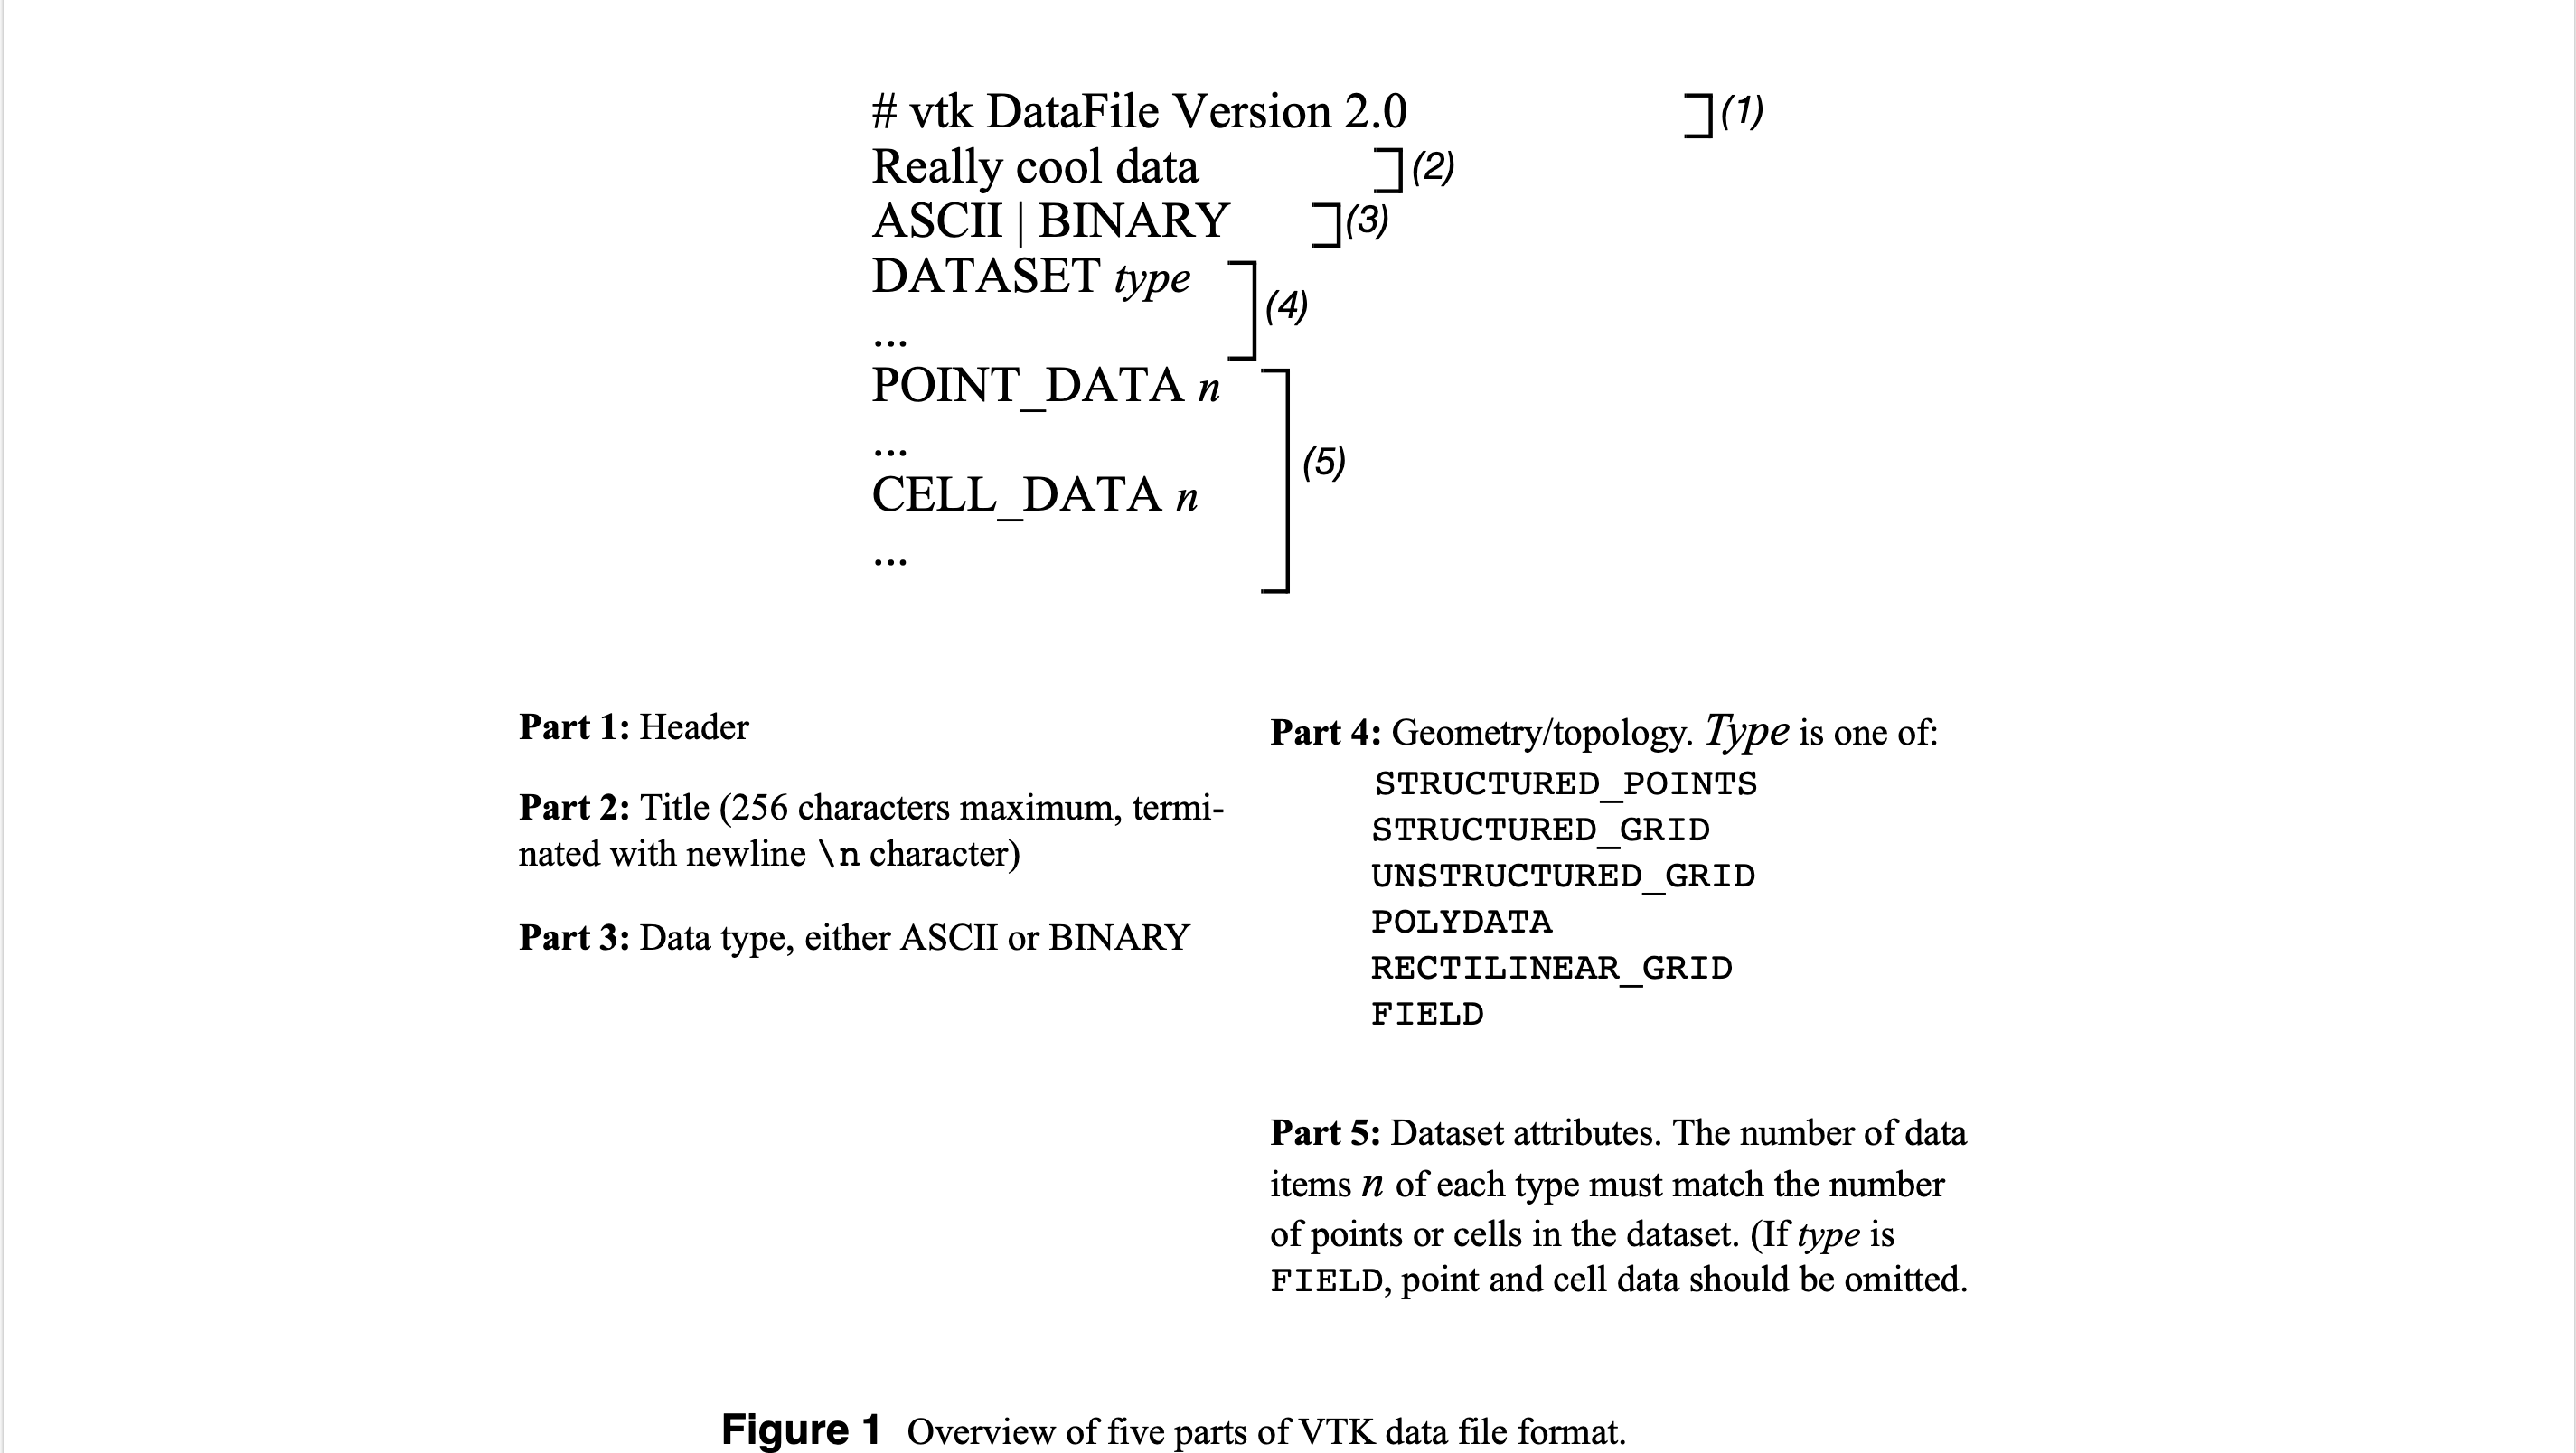
\includegraphics[width=50em]{./source/1.png}
}

\paragraph{\quad}在描述数据文件格式前请注意一下几点。
\begin{itemize}
    \item dataType是bit,unsigned_char,char,unsigned_short,unsigned_int,int,unsigned_long,long,
          float或者double其中之一。这些关键字用于描述数据的形式,既为了从文件中读取数据也为构建合适的
          内部数据对象。并非所有类都支持所有的数据类型。
    \item 无论是ASCII文件还是二进制文件,所有的关键字短语都是以ASCII形式编写。文件的二进制部分(如果在二进制部分)是
          是数据正确的,即定义点坐标、标量、单元索引等的数字(是正确的)。
    \item 索引是0偏移的,即第一个点id是0.
    \item 如果数据属性和几何/拓扑部分同时在一个文件中,那么在数据属性部分中的数值数量必须与几何/拓扑部分
          中定义的点或单元数量相等。
    \item 单元类型或索引是int类型。
    \item 二进制数据必须紧接前一个ASCII关键字和参数序列中的换行(\n)字符之后放入文件中。
    \item 几何拓扑描述必须出现在数据属性描述之前。
\end{itemize}

\paragraph{二进制文件}只要满足两个条件,二进制文件就可以在不同电脑系统之间移植。第一保证数据的字节序正确;其次
                    确保每个数据类型的长度一致。
\paragraph{\quad}大部分时候,vtk为你管理二进制文件的字节序。当你在一个电脑中写一个二进制文件,并从另外一个电脑
                中读取,表示数据的字节必要时将会自动转换。例如,在Sun架构中二进制文件以大端序写入,而在PC(译者注:应该是x86架构中)
                是以小端序储存的。这就导致在Sun工作站写入的文件需要在PC中读入时进行字节转换(见类vtkByteSwap的实现细节)。此处
                描述的vtk数据文件是以大端序形式写入的。
\paragraph{\quad}然而,一些文件格式没有显式地定义字节序形式。你将会发现根据初始系统的不同,外部程序或者类vtkVolume16Reader,vtkMCubesReader以及
                vtkMCubesWriter读写的数据可能会有不同的字节顺序。在这种情况下,vtk允许你使用以下方法指定字节序:
\begin{verbatim}
    SetDataByteOrderToBigEndian()
    SetDataByteOrderToLittleEndian()
\end{verbatim}
二进制文件的另外一个问题是操作系统可能使用不同字节数表示整数或其他原生类型。例如,某些64位操作系统可能8个字节表示一个整数,而其他操作
系统使用4个字节。目前vtk无法在不兼容数据长度的操作系统间转移二进制文件。在这种情况下,请改用ASCII文件格式。

\paragraph{数据集格式}可视化工具包(vtk)支持五种不同的数据集格式:结构化点,结构化网格,直线网格,非结构化网格和多边形数据。
            具有隐式拓扑的数据(结构化数据,如vtkImageData和vtkStructuredGrid)按x增加最快的顺序排列,然后是y,然后是z。
            这些格式如下。

\begin{itemize}
    \item {
        结构化点 \\
        该文件格式支持一维,二维和三维的结构化点数据集。其dimensions值$n_x,n_y,n_z$必须大于等于1.其spacing(间距)值
        必须大于0.(注:在版本1.0的数据文件中,spacing(间距)被称为“长宽比”,ASPECT_RATIO在版本2.0的数据结构中仍可使用,
        但不建议) \\
        \begin{verbatim}
            DATASET STRUCTURE_POINTS 
            DIMENSIONS nx ny nz
            ORIGIN x y z
            SPACING sx sy sz
        \end{verbatim}
    }
    \item {
        结构化网格 \\
        该文件格式支持一维,二维和三维的结构化网格数据集。其dimensions值$n_x,n_y,n_z$必须大于等于1.点坐标在POINTS节中
        的数据定义。其包含了每点的x-y-z数值。
        \begin{verbatim}
            DATASET STRUCTURE_GRID
            DIMENSIONS nx ny nz
            POINTS n dataType
            p0x p0y p0z
            p1x p1y p1z
            ...
            p(n-1)x p(n-1)y p(n-1)z
        \end{verbatim}
    }
    \item {
        直线型网格 \\
        直线型网格定义了具有规则拓扑和沿x-y-z坐标轴对齐的半规则拓扑数据集。几何由三个单调递增的坐标值列表定义,每个列表
        分别代表x-y-z坐标轴。其拓扑由指定的网格维度定义,其必须大于等于1.
        \begin{verbatim}
            DATASET RECTILINEAR_GRID
            DIMENSIONS nx ny nz
            X_COORDINATES nx dataType
            x0 x1 ... x(nx-1)
            Y_COORDINATES ny dataType
            y0 y1 ... y(ny-1)
            Z_COORDINATES nz dataType
            z0 z1 ... z(nz-1)
        \end{verbatim}
    }
    \item {
        多边形数据 \\
        多边形数据集由曲面图形图元顶点(和多边形顶点),直线(和折线),多边形
        (各种类型)和三角形的任意组合组成。多边形数据由POINTS,VERTICES,LINES,
        POLYGONS或者TRIANGLE_STRIPS部分定义。POINTS的定义与我们看到的结构化
        网格的定义相同。VERTICES,LINES,POLYGONS或者TRIANGLE_STRIPS关键词定义了
        多边形数据集拓扑。每一个这样的关键词需要两个参数:单元数n和单元列表的大小size。
        单元列表大小是表示列表所需的所有整数值。(例如,每个单元的numPoints之和与连通性指数)
        VERTICES,LINES,POLYGONS或者TRIANGLE_STRIPS不是必须的。
        \begin{verbatim}
            DATASET POLYDATA
            POINTS n dataType
            p0x p0y p0z
            p1x p1y p1z
            ... 
            p(n-1)x p(n-1)y p(n-1)z 

            VERTICES n size
            numPoints0,i0,j0,k0,...
            numPoints1,i1,j1,k1,... 
            ... 
            numPointsn-1,in-1,jn-1,kn-1,... 

            LINES n size 
            numPoints0,i0,j0,k0,...
            numPoints1,i1,j1,k1,... 
            ... 
            numPointsn-1,in-1,jn-1,kn-1,...

            POLYGONS n size 
            numPoints0,i0,j0,k0,...
            numPoints1,i1,j1,k1,... 
            ... 
            numPointsn-1,in-1,jn-1,kn-1,...

            TRIANGLE_STRIPS n size 
            numPoints0,i0,j0,k0,...
            numPoints1,i1,j1,k1,... 
            ... 
            numPointsn-1,in-1,jn-1,kn-1,...
        \end{verbatim}
        \item {
            非结构化网格 \\
            非结构化网格数据集包含任意可能的单元类型的组合。非结构化网格由点,单元和单元类型定义。
            CELLS关键字要求两个参数:单元数n和单元列表的大小size。单元列表大小是表示列表所需的所有整数值(例如,
            每个单元的numPoints之和与连通性指数)。CELL_TYPE关键字要求一个参数:单元数n。这个值应与CELLS关键词
            指定的值相匹配。单元类型数据是每个单元一个指定单元类型的整数值(见vtkCell.h或图二)
            \begin{verbatim}
                DATASET UNSTRUCTURED_GRID
                POINTS n dataType
                p0x p0y p0z
                p1x p1y p1z
                ...
                p(n-1)x p(n-1)y p(n-1)Z

                CELLS n size
                numPoints0,i,j,k,l,... 
                numPoints1,i,j,k,l,...
                numPoints2,i,j,k,l,... 
                ... 
                numPointsn-1,i,j,k,l,... 

                CELL_TYPE n
                type0
                type1
                type2
                ... 
                typen-1
            \end{verbatim}
        }
        \item{
            场 \\
            场数据是没有拓扑和几何结构的通用数据格式,也没有特定维度。通常,场数据和数据集的点或单元相关联。然而,如
            果指定FIELD类型为数据集类型(见图一),那么就定义了通用vtk数据对象。使用下节介绍的格式定义场。也可见在158页的“Working
            With Field Data"和在7页的“Examples”章节的第四个例子。
        }
    }
\end{itemize}


\end{document}